% QUESTO E' IL MODELLO DI DOCUMENTO FINALE DA PRESENTARE ALLA PROVA D'ESAME DI
% "SISTEMI INFORMATIVI" A.A. 2014/2015. E' BASATO SUL MODELLO ADOTTATO DA
% SPRINGER PER GLI ATTI DELLE PROPRIE CONFERENZE, COME SPIEGATO NEL SEGUITO. 

\documentclass{llncs}

% Si utilizzi il pacchetto babel se si scrive in italiano
\usepackage[italian]{babel}
\usepackage[applemac]{inputenc}
\usepackage{algorithmicx}
\usepackage{algpseudocode}
\usepackage{geometry}
\usepackage{graphicx}
\usepackage{caption}
\usepackage{hyperref}
\usepackage{subcaption}
\usepackage{mathtools}
\usepackage{float}

% \usepackage[caption=false]{subfig}

\begin{document}

\title{Documento finale per la prova d'esame di Sistemi Informativi
  a.a. 2014/2015} 
\author{
	Catalin Copil\\\email{catalin.copil@studenti.unipd.it}\\ 
	Mattia de Stefani\\\email{mattia.destefani@studenti.unipd.it}\\ 
	Giulio Lovisotto\\\email{giulio.lovisotto@studenti.unipd.it}} 
\institute{}

\date{\today}
% Just remember to make sure that the TOTAL number of authors
% is the number that will appear on the first page PLUS the
% number that will appear in the \additionalauthors section.

\maketitle
\begin{abstract}
Il presente documento descrive le attivit\`a di laboratorio svolte dagli autori (gruppo 12) durante il corso di Sistemi Informativi, tenuto dal professor M. Melucci presso l'Universit\`a di Padova, anno accademico 2014/2015. 
L'obiettivo delle tecniche utilizzate \`e quello di massimizzare l'efficacia della funzione di reperimento nella collezione di articoli scientifici CACM. All'interno di questo documento vengono riportate informazioni sulle scelte implementative dei metodi di Information Retrieval trattati. I componenti del gruppo hanno deciso di integrare nel reperimento le tecniche proposte scegliendo di partire da \textsc{bm25} come riferimento. In particolare, sono stati integrati gli algoritmi di \textsc{pagerank}, \textsc{relevance feedback}, \textsc{lsa}, \textsc{hits}. Inoltre ai fini dell'ottimizzazione \`e stato utilizzata un Evolution Strategy. Il documento comprende un'analisi ragionata dei risultati ottenuti, e termina con alcune conclusioni generali sul lavoro svolto.

%Questo documento illustra il perscorso effettuato per arrivare ad ottenere una buona conoscenza del ramo dell'Information Retrieval.
%Partendo dalle conoscenze di base ad ogni esercitazione è stato aggiunto un tassello, il quale non è altro che un'attributo in più da considerare per il calcolo della precisione dei file ritenuti da noi importanti.
%All'interno del documento saranno spiegati i diversi progetti effettuati. Come siamo passati da un'indicizzazione manuale ad una automatica (laboratorio 2), l'algoritmo di reperimento implementato per effettuare il ranking dei documenti presenti nella collezione per ogni richiesta, query (laboratorio 3). L'introduzione dei giudizi di rilevanza e la loro influenza sul risultato elaborato dall'algoritmo di reperimento scelto (laboratorio 4). Il calcolo effettuato del pagerank di ogni documento e come quest'ultimo in fluisca sul ranking (laboratorio 5). L'analisi della relazione tra una collezione di documenti e i termini contenuti in essi tramite l'utilizzo della tecnica \textbf{LSA} (laboratorio 6 ). Concludento con l'introduzione e lo studio di \textbf{HITS} (Hyperlink-Induced Topic Search): algoritmo di analisi dei link (laboratorio 7).  
	
	
\end{abstract}

\section{Introduzione}
\label{sec:introduzione}

% Introdurre brevemente lo scopo del corso.
Il corso di Sistemi Informativi ha come obiettivo l'insegnamento di nozioni basilari di Information Retrieval e Motori di Ricerca. Gli argomenti trattati a lezione ed i concetti applicati durante i vari laboratori sono stati utili a comprendere il funzionamento di un reale sistema di Information Retrieval.

Il progetto svolto nelle lezioni di laboratorio prevede l'utilizzo di una collezione di dati fornita dal docente; la collezione utilizzata \'e una raccolta di articoli scientifici tratti dalla rivista \textit{Communications of the ACM} (http://cacm.acm.org/)
La collezione di documenti \'e stata fornita come un unico file xml dove ogni nodo di documento contiene un identificativo, un titolo e altre informazioni come abstract, autori, luogo, riferimenti e citazioni ad altri documenti della collezione.
Oltre al file contenente i documenti sono stati forniti file contenenti le parole chiave sotto forma di stem, un insieme di query e l'insieme delle citazioni tra i documenti.

%Durante le lezioni di laboratorio gli studenti, organizzati in piccoli gruppi, hanno avuto modo di implementare diverse tecniche nel proprio progetto che ....

\vspace{30px}
Che collezione usiamo (http://ir.dcs.gla.ac.uk/resources/test\_collections/cacm/). No stop words, no stemming (gia fatto). 
Abbiamo a disposiz il grafo delle citazioni quindi useremo \textsc{pagerank} e Hits (link analysis), spiegare brevemente cosa sono questi. Spiegare LSA. Spiegare ES. Related works?  citt\`e
\subsection{Organizzazione}
In sezione .. spiegeremo .., in sezione .. spiegheremo .. etc.

%Quando si scrive l'introduzione, si deve tenere presente che il lettore atteso
%sar\`a a conoscenza degli elementi di base. Si dovranno quindi introdurre i
%concetti non normalmente trattati in un corso di base in Information Retrieval e
%che sono invece utilizzati nel proprio documento.
%
%Il resto del documento sar\`a scritto con i criteri seguenti:
%\begin{itemize}
%\item esaustivit\`a
%\item precisione
%\item chiarezza
%\item correttezza
%\item sintesi
%\end{itemize}


\section{Metodologia}
\label{sec:metodologia}

Spiegare notazione grafo, parametri, usiamo 1 simbolo per indicare gli score. Quando scriviamo una sezione qui sotto 2.x, se ci serve della notazione poi andiamo a metterla qui. 
Fare dei paragrafi per BM25, PageRank, Hits, LSA, ES.

%In questo paragrafo, si illustreranno i metodi sviluppati e sperimentati con le
%attivit\`a di laboratorio. Le notazioni e tutti gli aspetti non banali dovranno
%essere spiegati. Naturalmente, la notazione di un paragrafo non dovr\`a essere
%reintrodotta nei paragrafi successivi, di conseguenza, la notazione non dovr\`a
%essere ambigua.

\subsection{Approccio}
\label{sec:approccio}

%Vogliamo max la map. Usando treceval spiegare cos'e'. Spiegare brevemente il lavoro, molto veloce dire che abbiamo lavorato insieme dopo la prima sessione in lab. Usato python, con \texttt{numpy} per matrici, matplotlib per plottare, networkx per grafi, git per versionamento, latex per i report.
%Il nostro scopo e' ottenere un valore di map il piu' elevato possibile. Per calcolarla e verificarne il cambiamento durante le varie versione del codice utilizziamo \texttt{treceval}, esso e' il tool standard usato dalla "TREC community" per valutare un'esecuzione ad hoc, dandole il file contenete i risultati e un set standard di risultati giudicati.  

%Abbiamo deciso di utilizzare un approccio probabilistico poiche' fornisce una formalizzazione piu' pulita di cosa volgiamo che faccia un sistema IR: dare documenti rilevanti agli utenti. 
%Inoltre per via delle nostre conoscenze abbiamo voluto utilizzare il linguaggio Python per dare corpo ai progetti. Inoltre vi sono diverse librerie che implementano molti metodi utili per tale corso e per garantire buone performance al codice: \texttt{numpy} usata per la gestione delle matrici, \texttt{matplotlib} utilizza per effettuare i plot (grafici) dei risultati ottenuti, \texttt{networkx} utilizzata per la creazione e gestione dei grafi.
%Oltre a \texttt{Python} abbiamo utilizzato altri software per il lavoro. E' stato usato \texttt{Git}, e' un sistema di versionamento distribuito, per lo scambio del codice e l'aggiornamente delle diverse versioni di quest'ultimo. Infini \texttt{latex} per la scrittura dei pdf di report.
%Per ogni esercitazioni è stato utilizzato un approccio di gruppo. Dopo la prima sessione di laboratorio di ogni esercitazione ci siamo ritrovati per la scrittura del codice, la discussione sui risultati e la stesione del report.

\subsection{Indicizzazione} \label{sec:metodi-di-indic}

Qui va il contenuto del laboratorio n. 2.

\subsection{Reperimento}
\label{sec:metodi-di-reper}

Qui va il contenuto del laboratorio n. 3. Esso rappresenta la \textit{baseline}.

\subsection{Relevance Feedback}
\label{sec:relevance-feedback}

Qui va il contenuto del laboratorio n. 4.

\subsection{PageRank}
\label{sec:pagerank}

Qui va il contenuto del laboratorio n. 5.

\subsection{Latent Semantic Analysis}
\label{sec:lsa}

Qui va il contenuto del laboratorio n. 6.

\subsection{Hyper-linked Induced Topic Search}
\label{sec:hits}

Qui va il contenuto del laboratorio n. 7.

\subsection{Evolution Strategy}
\label{sec:es}

Per ottimizzare gli algoritmi di reperimento abbiamo scelto di utilizzare un Evolution Strategy~\cite{back1996evolutionary} (ES) che e' una tecnica di ottimizzazione basata sui principi che regolano l'evoluzione. Tecniche di questo tipo sono piu' robuste rispetto ai metodi di ricerca lineare per quanto riguardo i massimi locali. Il loro svantaggio consiste nel maggior numero di valutazioni richieste. Nel nostro contesto una valutazione impiega circa 3-10 secondi a seconda della complessita' del metodo di reperimento. Cio' permette di eseguire l'algoritmo di ottimizzazione in un tempo accettabile.

I parametri che abbiamo scelto di ottimizzare cambiano in base alla tecnica di reperimento (e quindi del laboratorio). Per il laboratorio 3 abbiamo scelto di ottimizzare $k_1, b$, ignoriamo $k_2$ in quando abbiamo visto che non ci sono termini ripetuti nelle query e quindi tale termine non influisce sul punteggio. Per il laboratorio 5 ottimizziamo $k_1, b, \alpha$. Per il laboratorio 7 ottimizziamo $k_1, b, \alpha, \beta, \gamma$. La funzione da massimizzare e' la Mean Average Precision.

Figura \ref{fig:es_all} riporta l'andamento della MAP durante l'ottimizzazione della funzione di reperimento dei laboratori. 
\begin{figure*}
        \centering
        \begin{subfigure}[b]{0.475\textwidth}
            \centering
            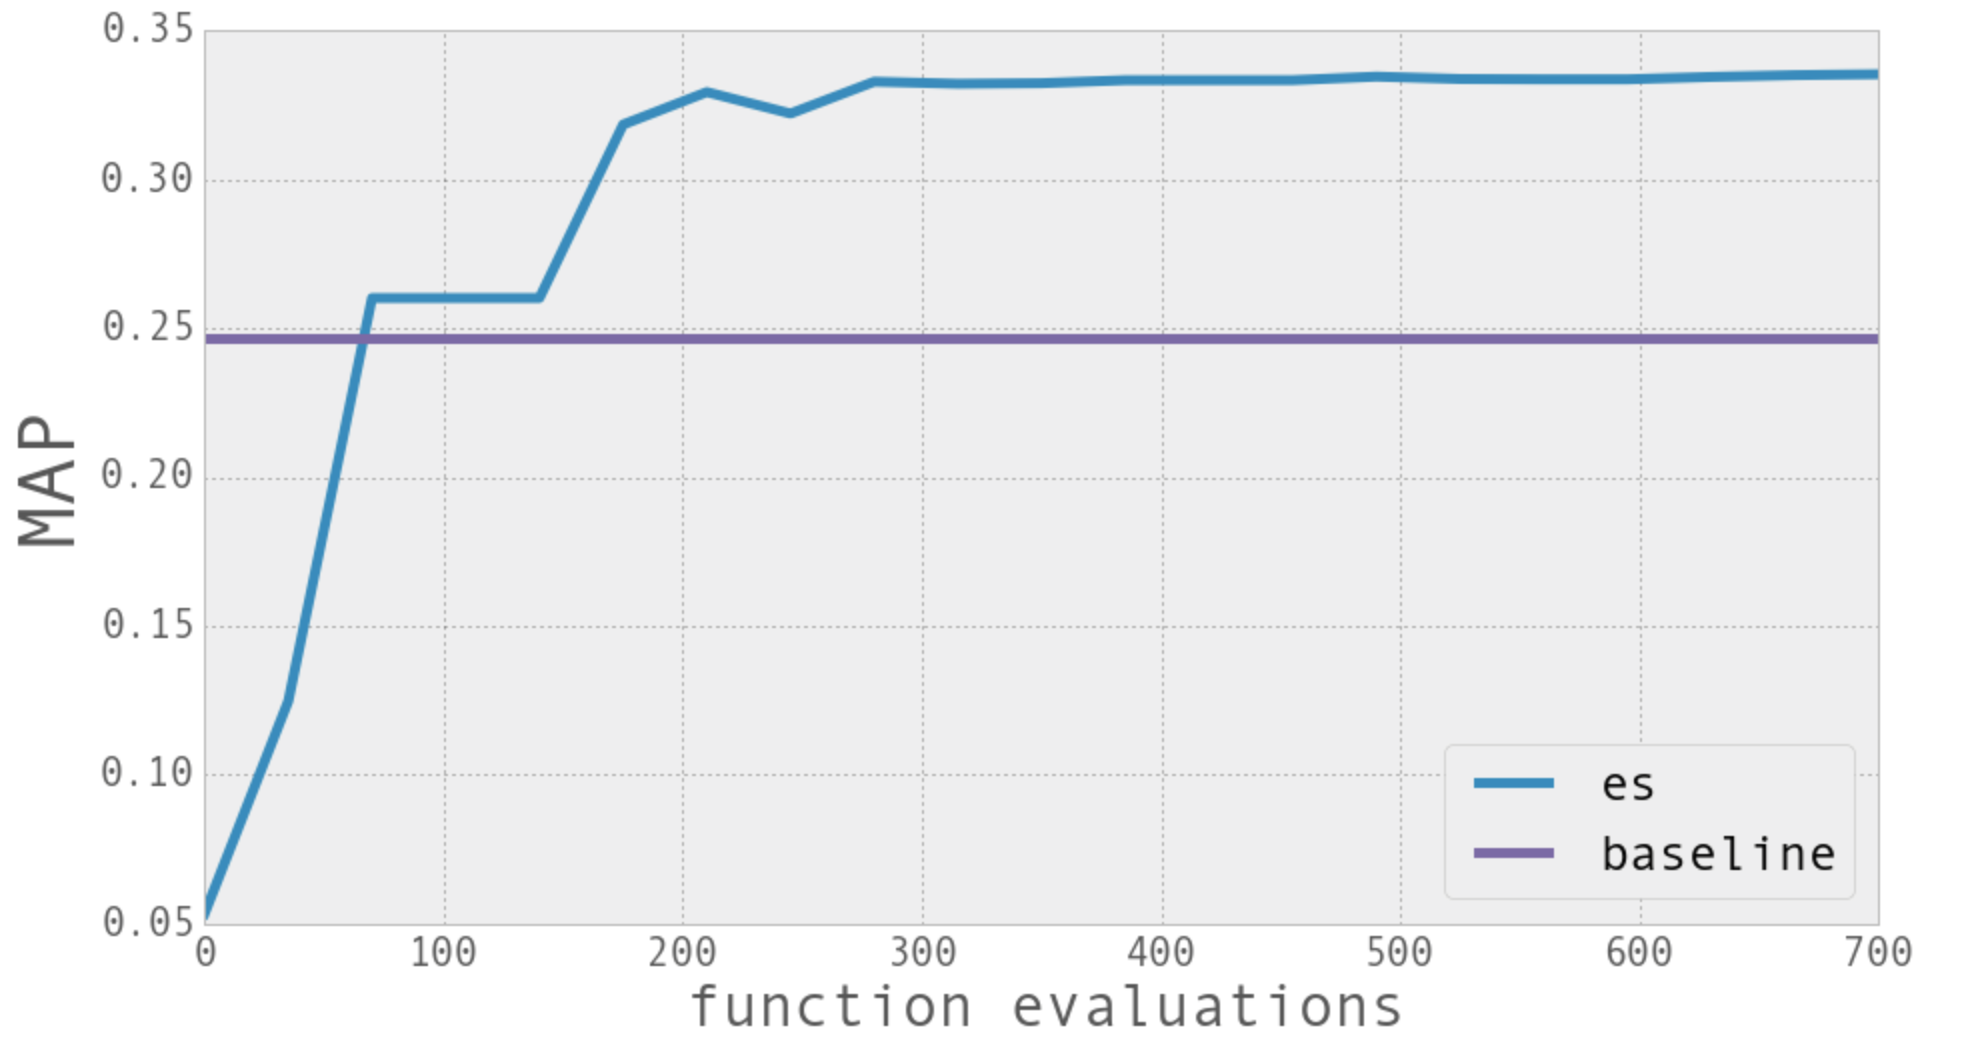
\includegraphics[width=\textwidth]{figures/es_lab3.png}
            \caption[Network2]%
            {{\small Laboratorio 3 (baseline)}}    
            \label{fig:es_lab3}
        \end{subfigure}
        \hfill
        \begin{subfigure}[b]{0.475\textwidth}  
            \centering 
            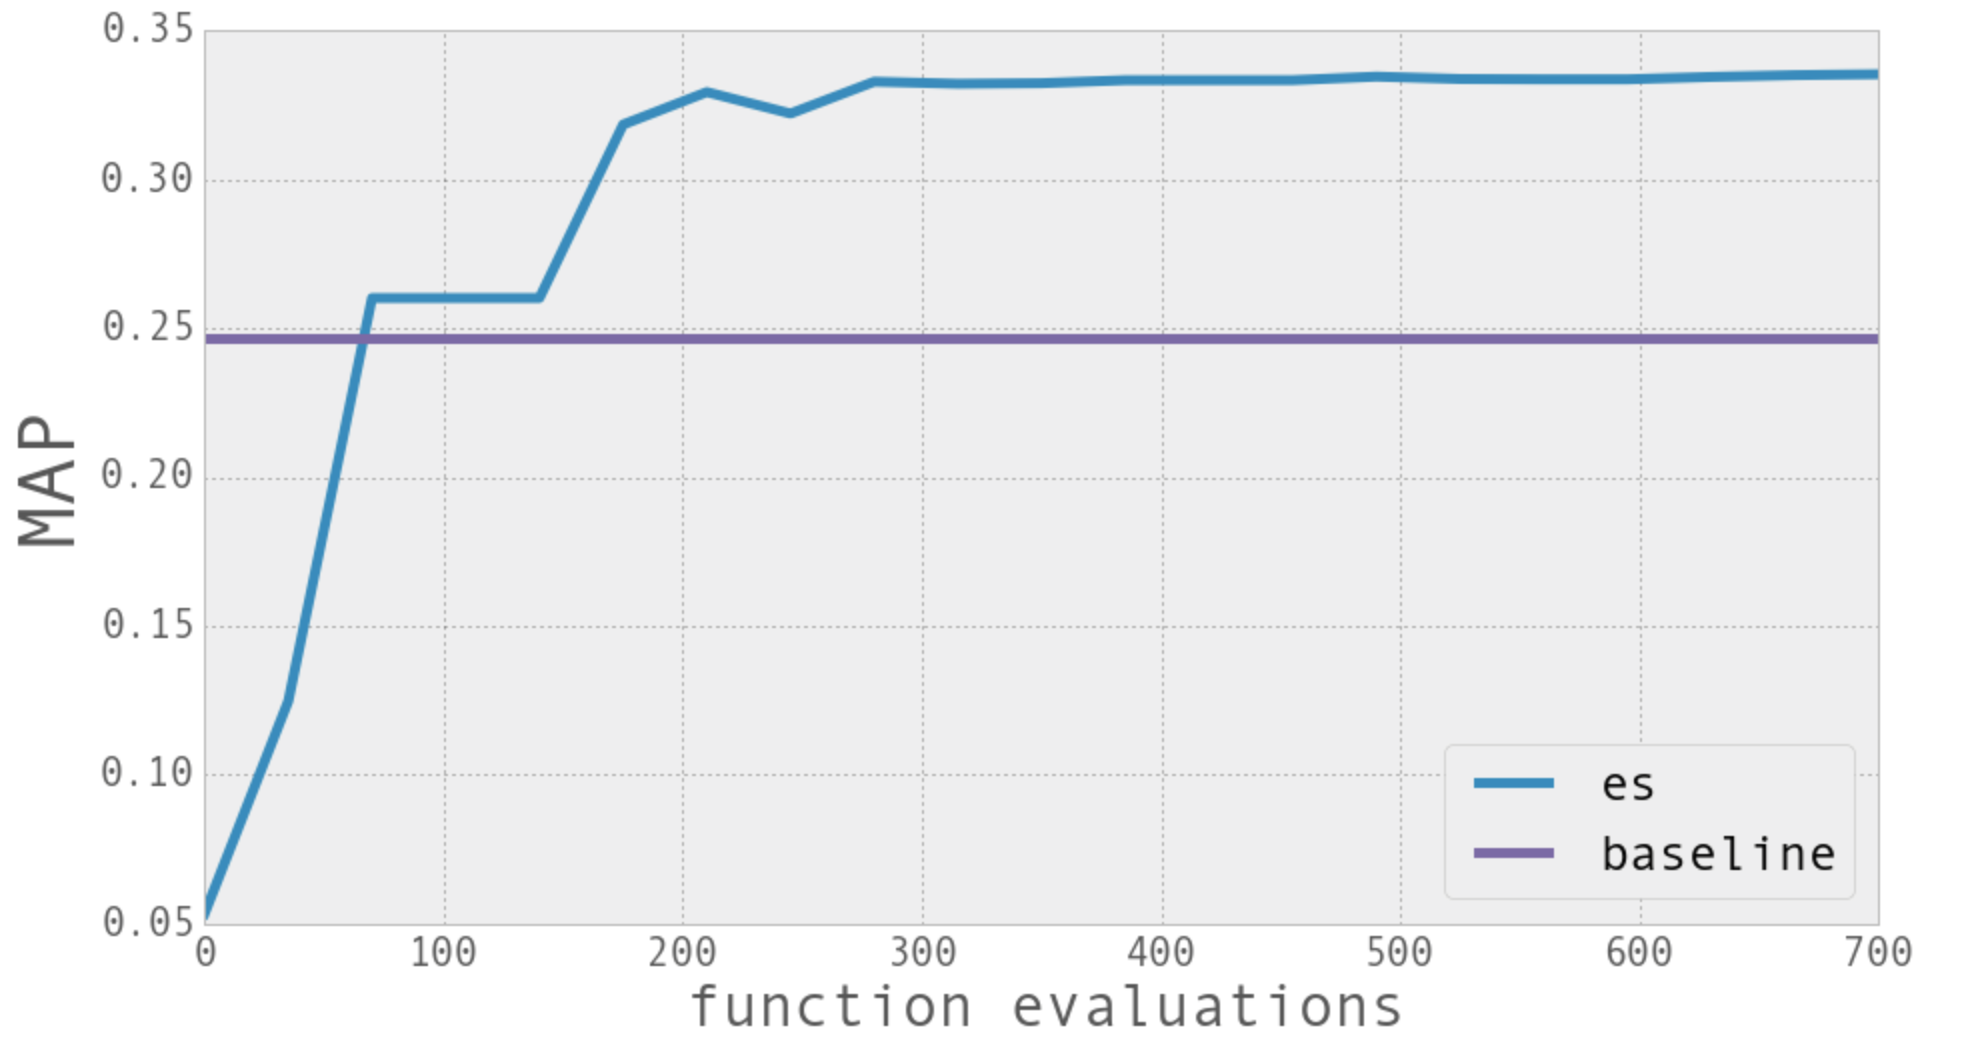
\includegraphics[width=\textwidth]{figures/es_lab3.png}
            \caption[]%
            {{\small Laboratorio 4 (relevance feedback esplicito)}}    
            \label{fig:es_lab4_esp}
        \end{subfigure}
        \vskip\baselineskip
        \begin{subfigure}[b]{0.475\textwidth}   
            \centering 
            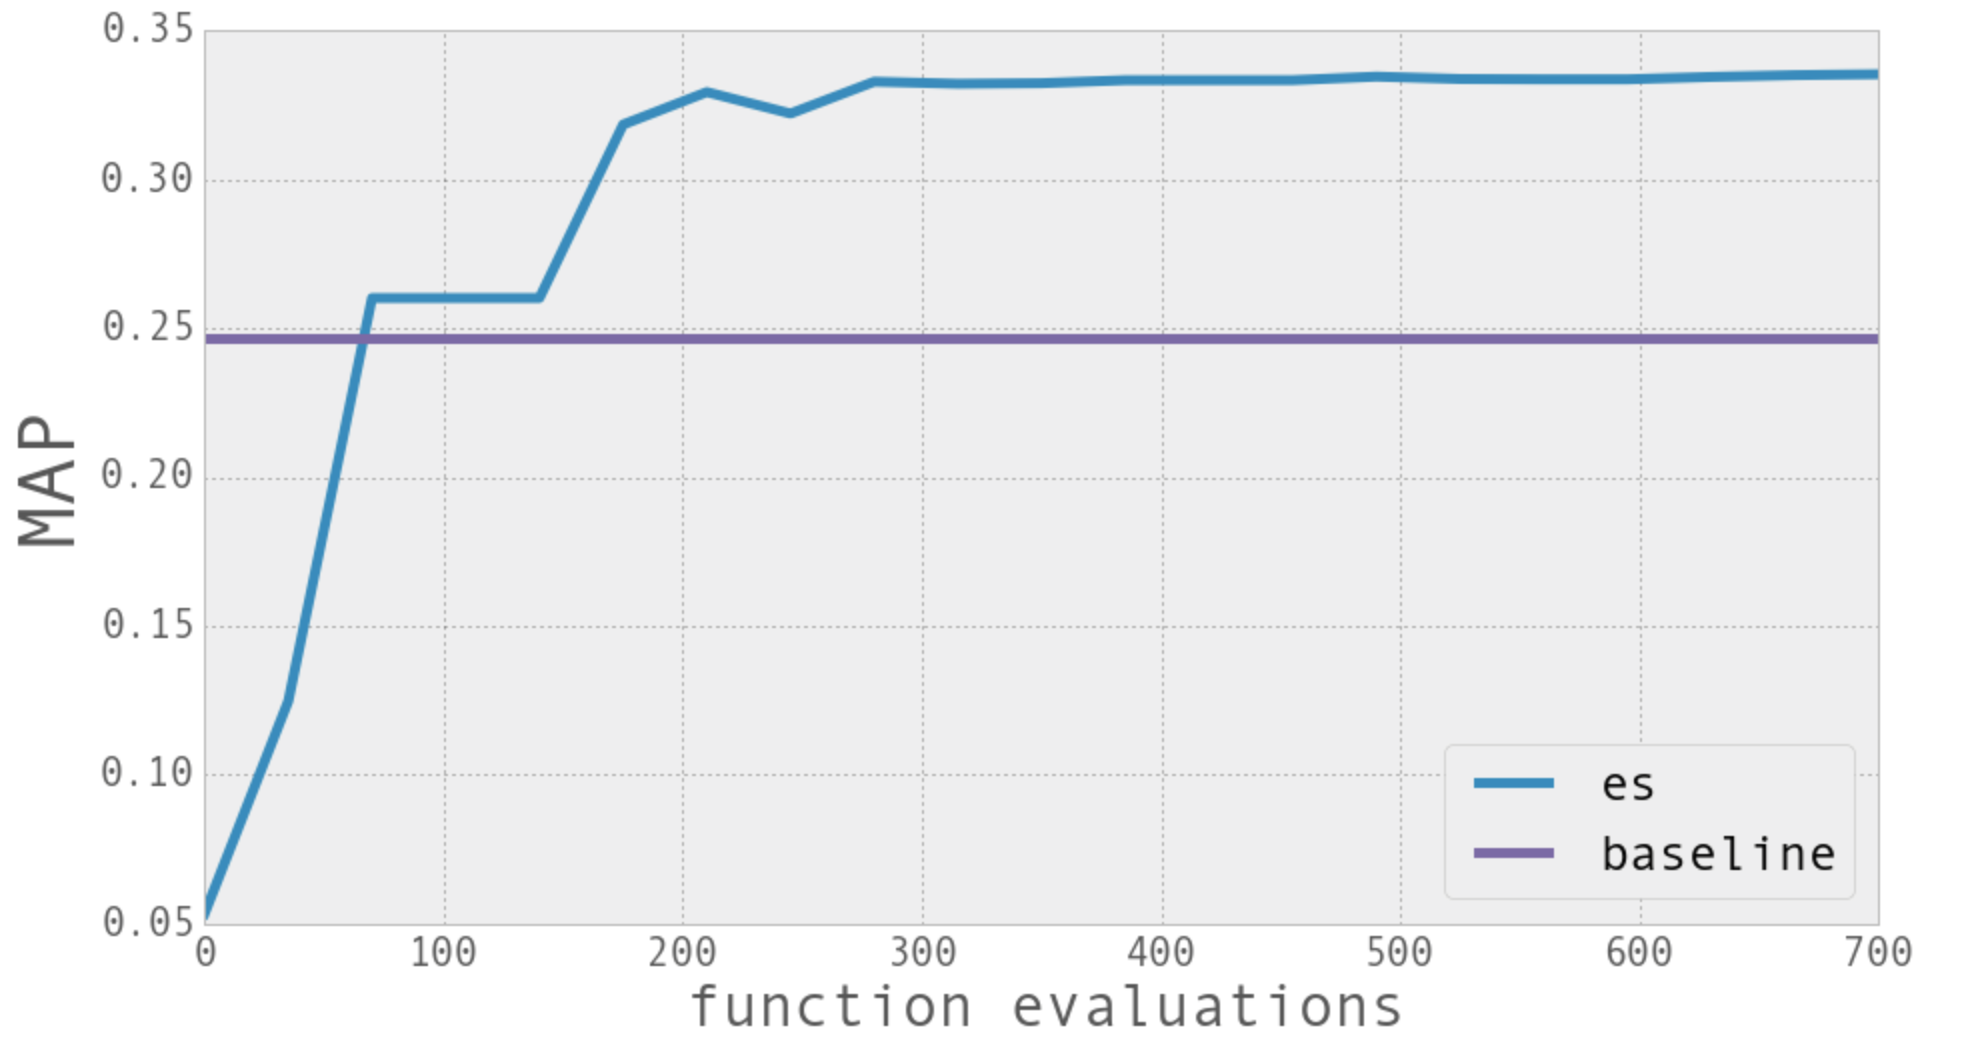
\includegraphics[width=\textwidth]{figures/es_lab3.png}
            \caption[]%
            {{\small Laboratorio 4 (relevance feedback pseudo)}}    
            \label{fig:es_lab4_pse}
        \end{subfigure}
        \quad
        \begin{subfigure}[b]{0.475\textwidth}   
            \centering 
            \includegraphics[width=\textwidth]{figures/es_lab5.png}
            \caption[]%
            {{\small Laboratorio 5 (\textsc{pagerank})}}    
            \label{fig:es_lab5_esp}
        \end{subfigure}
        \vskip\baselineskip
        \begin{subfigure}[b]{0.475\textwidth}  
            \centering 
            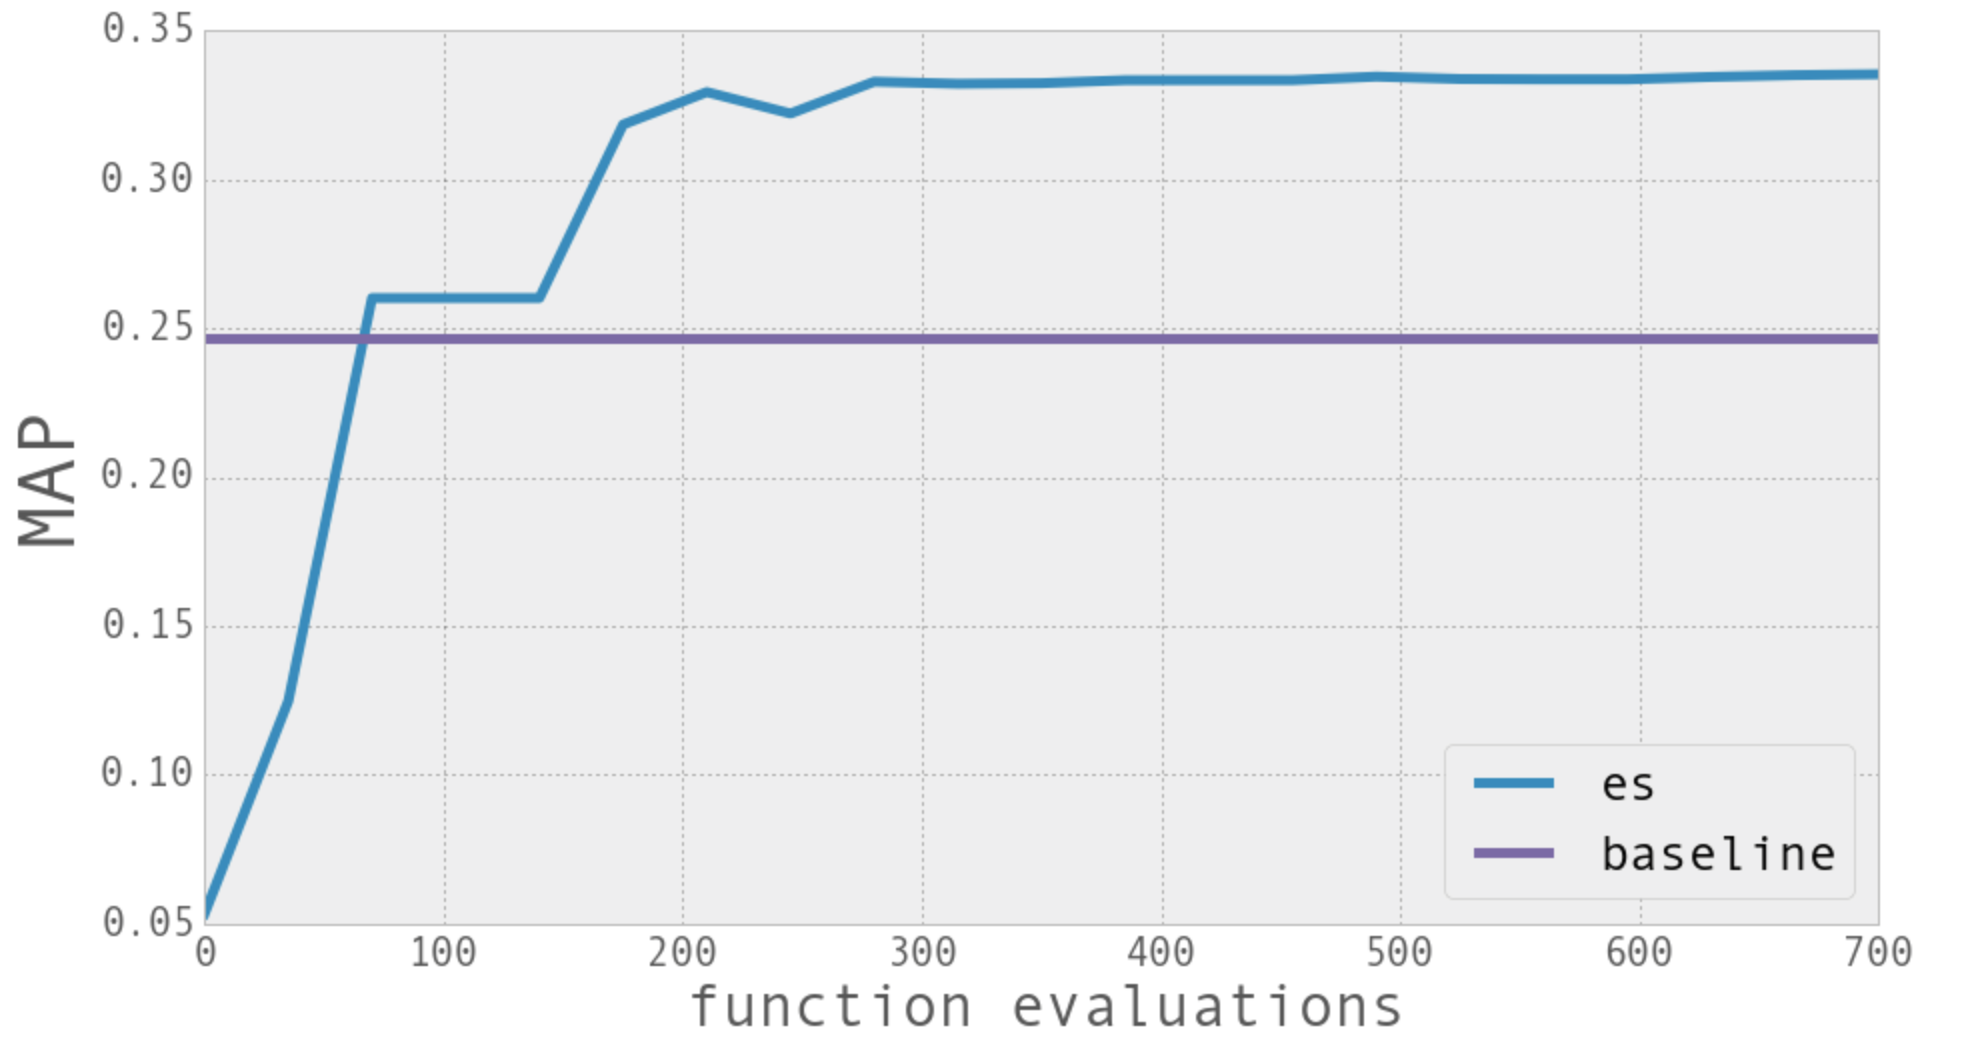
\includegraphics[width=\textwidth]{figures/es_lab3.png}
            \caption[]%
            {{\small Laboratorio 6 (\textsc{lsa})}}    
            \label{fig:es_lab6}
        \end{subfigure}
        \quad
        \begin{subfigure}[b]{0.475\textwidth}   
            \centering 
            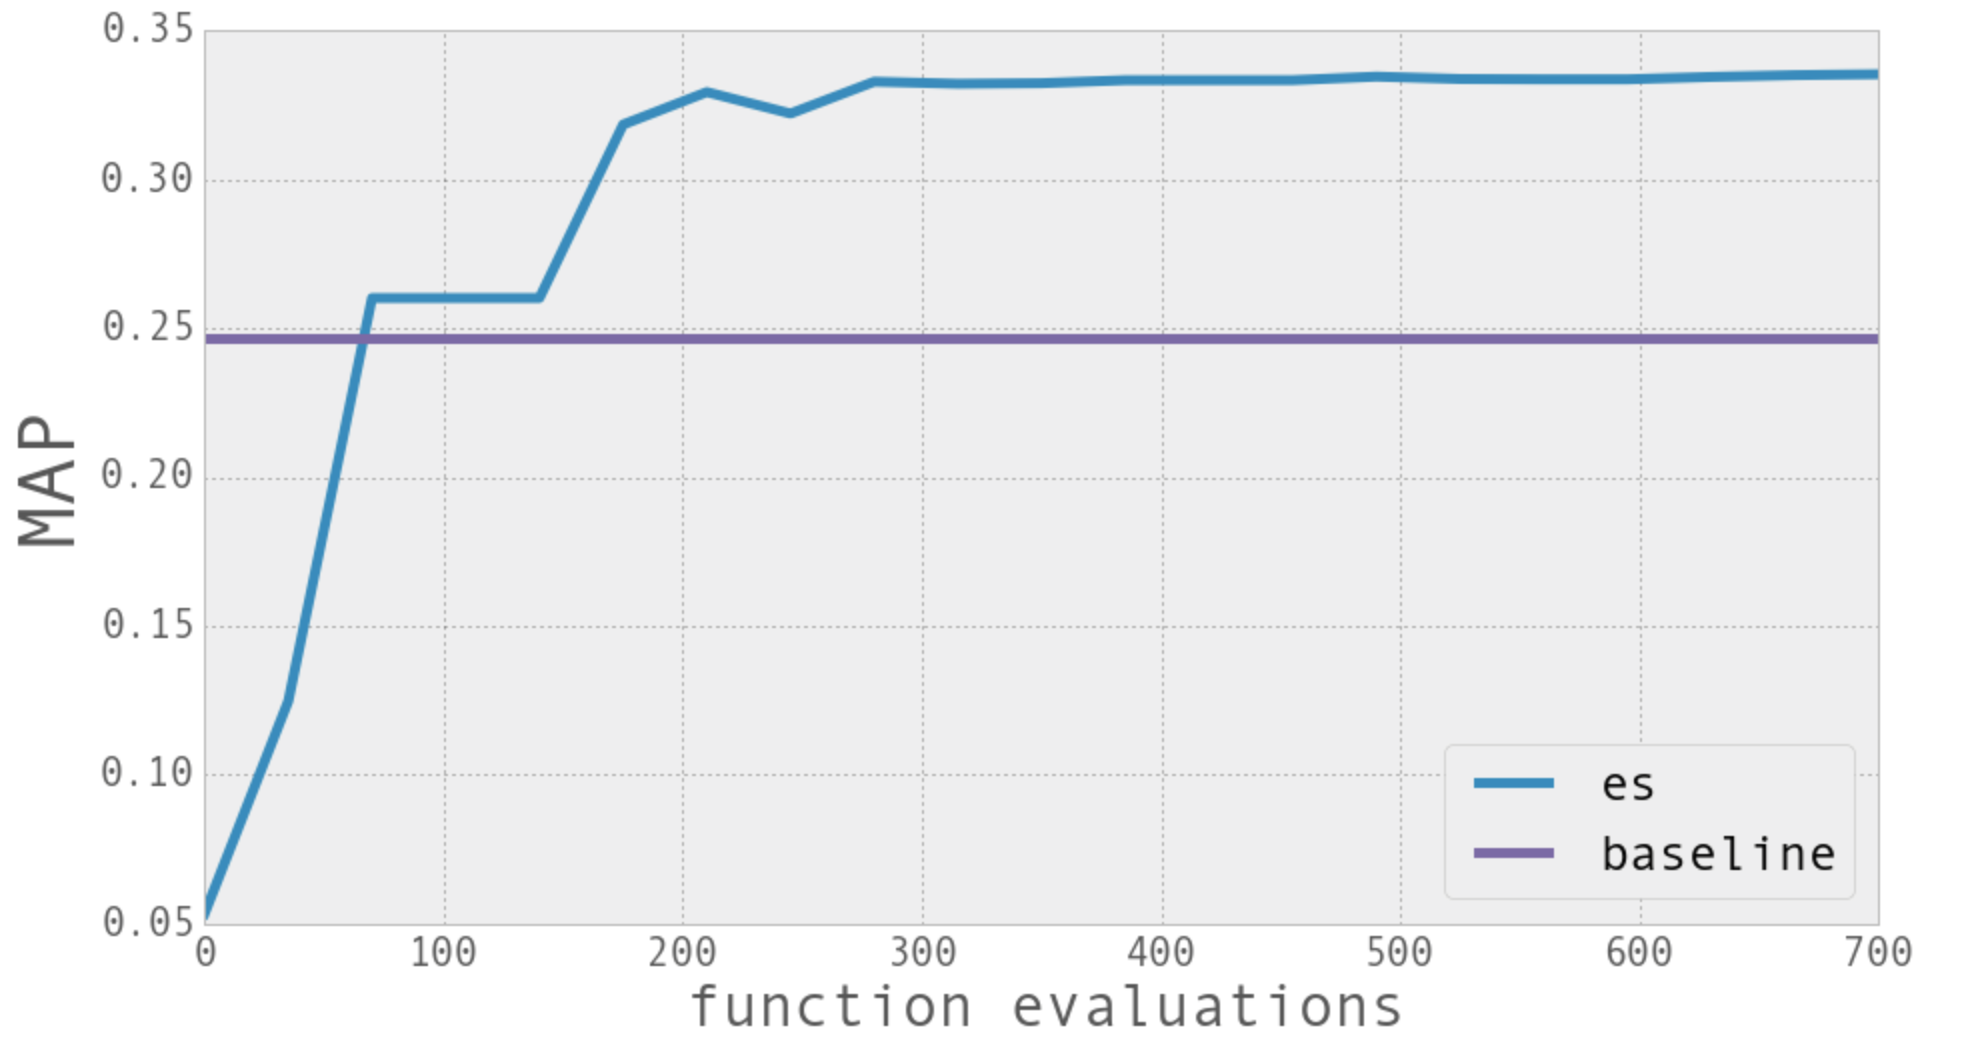
\includegraphics[width=\textwidth]{figures/es_lab3.png}
            \caption[]%
            {{\small Laboratorio 7 (\textsc{hits})}}    
            \label{fig:es_lab7}
        \end{subfigure}
        \caption[ The average and standard deviation of critical parameters ]
        {\small The average and standard deviation of critical parameters: Region R4} 
        \label{fig:es_all}
\end{figure*}


%\begin{figure}
%	\centering
%	\begin{subfigure}{.5\textwidth}
%		\centering
%		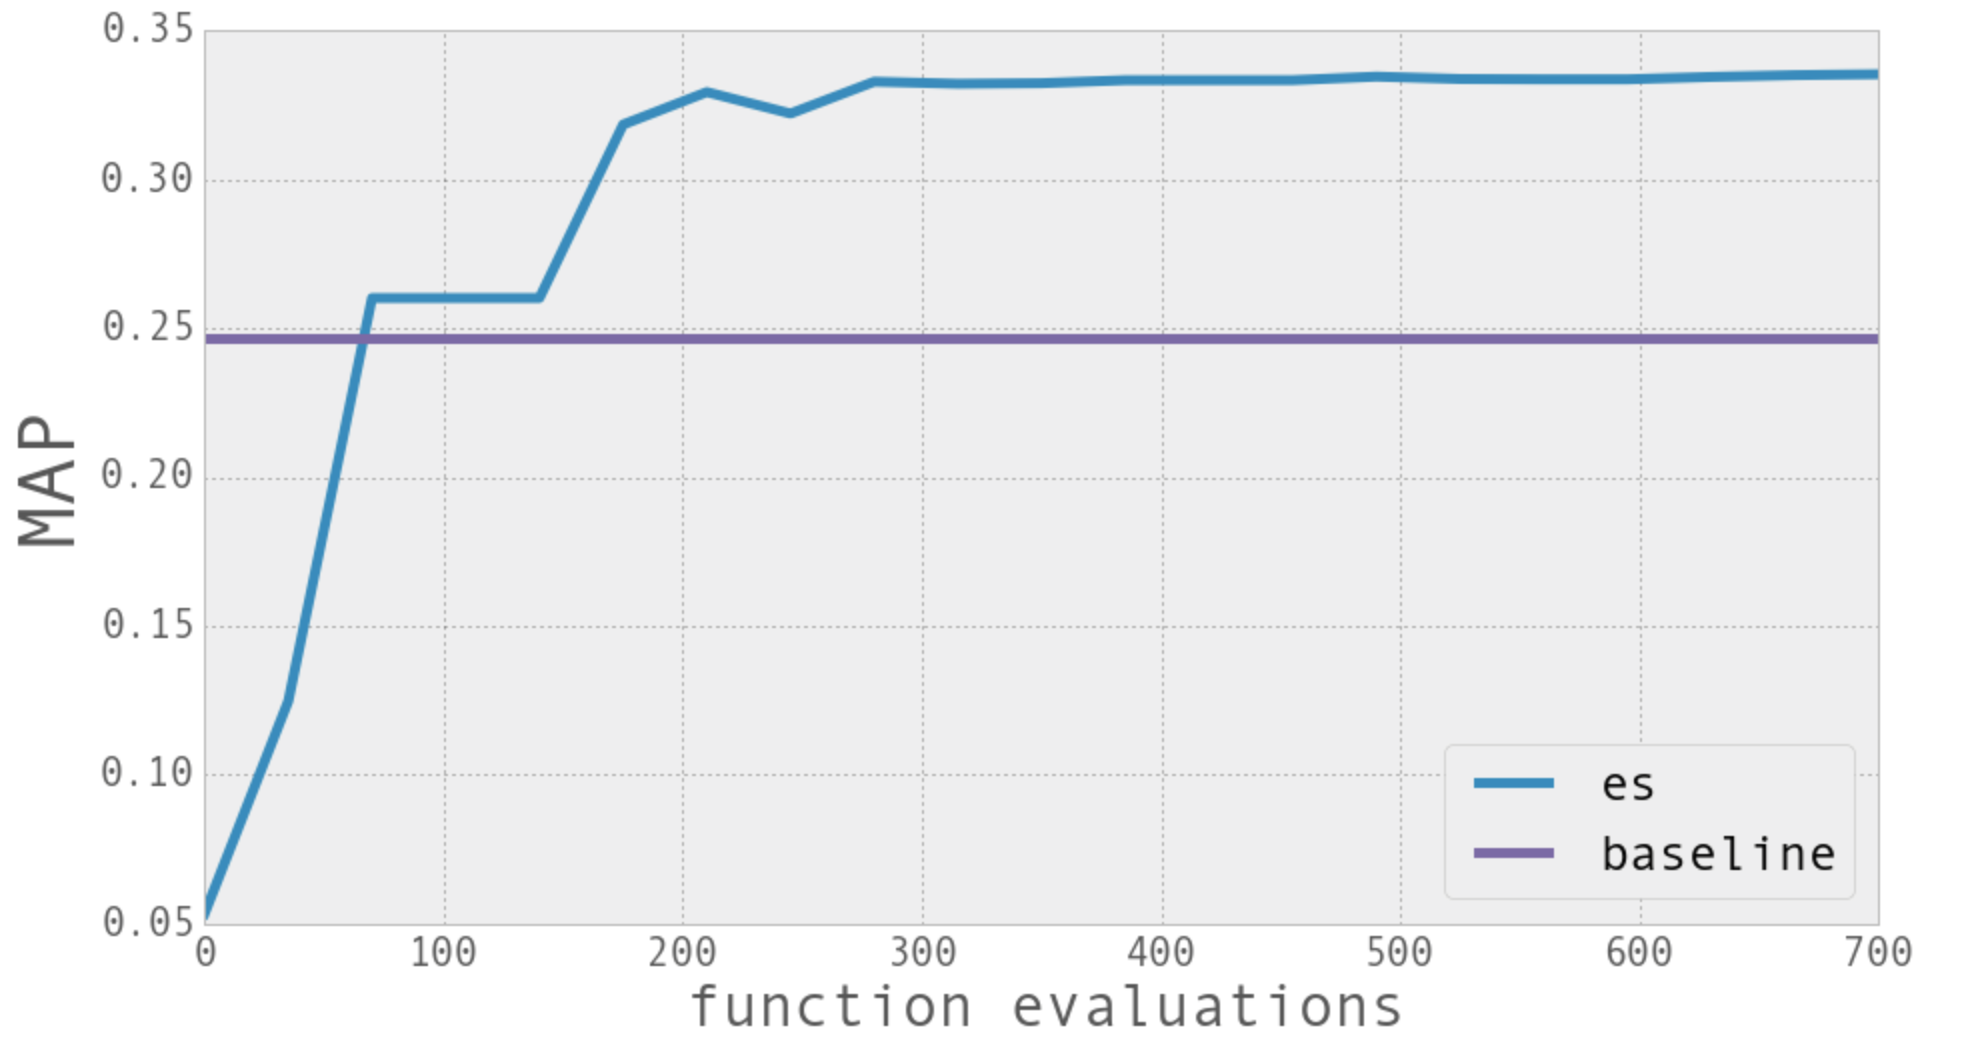
\includegraphics[width=1\textwidth]{figures/es_lab3.png}
%		\caption{MAP durante iterazioni dell'ES per il laboratorio 3.}
%		\label{fig:uno}
%	\end{subfigure}%
%	\begin{subfigure}{.5\textwidth}
%		\centering
%		\includegraphics[width=1\textwidth]{figiures/es_lab5.png}
%		\caption{Grafo base ($B_{56}$).}
%		\label{fig:due}
%	\end{subfigure}
%	\caption{MAP durante iterazioni dell'es}
%	\label{fig:unodue}
%\end{figure}

\begin{figure}[htbp]
	\begin{center}
		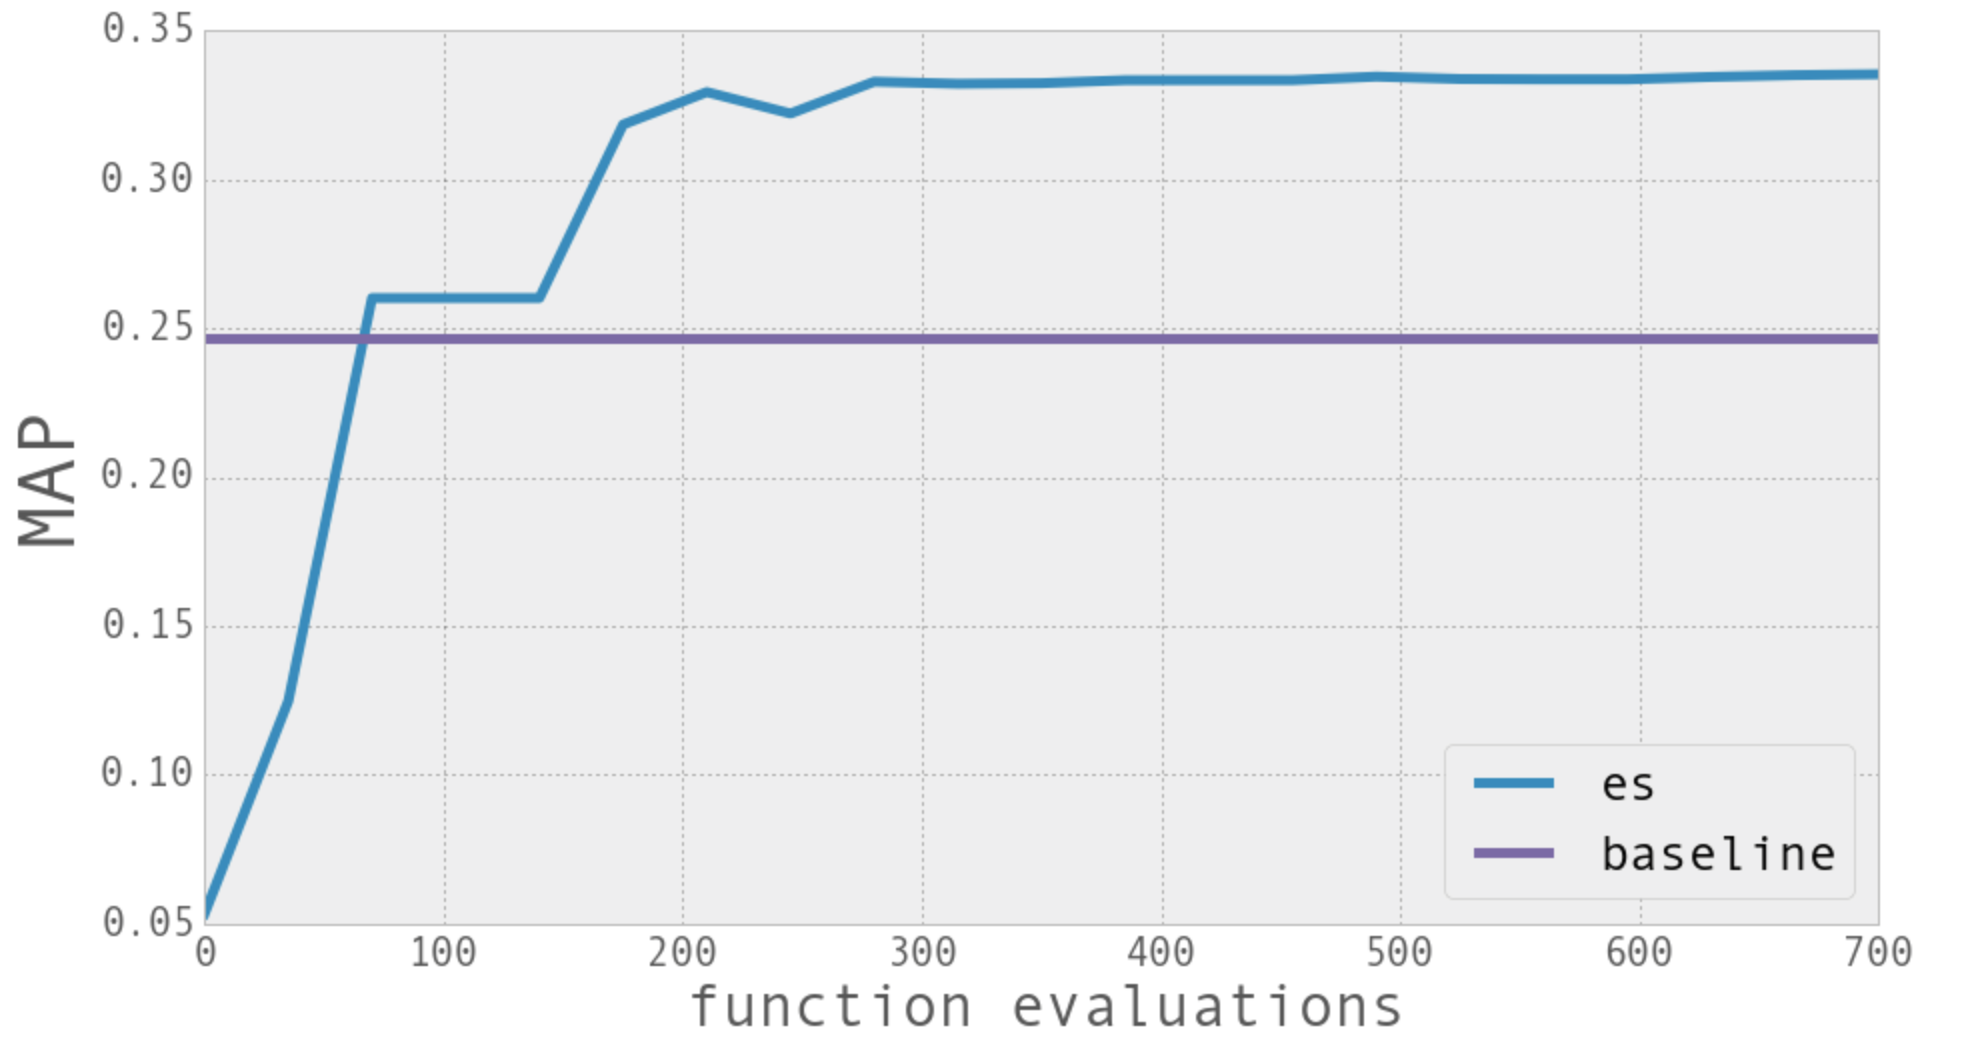
\includegraphics[width=0.75\textwidth]{figures/es_lab3.png}
		\caption{MAP durante ottimizzazione laboratorio 3.}
		\label{fig:es_lab3}
	\end{center}
\end{figure}
\begin{figure}[htbp]
	\begin{center}
		\includegraphics[width=0.75\textwidth]{figures/es_lab5.png}
		\caption{MAP durante ottimizzazione laboratorio 5.}
		\label{fig:es_lab5}
	\end{center}
\end{figure}
\begin{figure}[htbp]
	\begin{center}
		\includegraphics[width=0.75\textwidth]{figures/es_lab5.png}
		\caption{MAP durante ottimizzazione laboratorio 7.}
		\label{fig:es_lab7}
	\end{center}
\end{figure}

Tabella \ref{tab:es} riporta i risultati dell'ottimizzazione.
\begin{table}[htdp]
\caption{Risultati ottimizzazione con ES per i vari laboratori.}
\begin{center}
\begin{tabular}{|c|c|c|}
\hline
laboratorio & parametri & MAP \\
 \hline
3 & $k_1 = 0.0253, b = 0.0221$ & $0.3354$ \\
5 & $k_1 = 0.0237, b = 0.0, \alpha=0.7832$ & $0.3366$ \\
7 & $k_1 = 0.0237, b = 0.0, \alpha=0.7832$ & $0.3366$ \\
\hline
\end{tabular}
\end{center}
\label{tab:es}
\end{table}

Come si puo' vedere grazie all'ES si e' ottenuto un notevole miglioramento in termini di MAP rispetto alla nostra prima versione. I risultati dell'ottimizzazione vengono discussi in Sezione \ref{sec:risult-sper}.

\subsection{Altri metodi}
tipo lucene
\label{sec:altri-metodi}

Se sono stati sviluppati altri metodi, descriverli qui.



\section{Risultati sperimentali}
\label{sec:risult-sper}

In questa sezione verranno discussi i risultati sperimentali dei vari laboratori. Per confrontare le diverse funzioni di reperimento la configurazione di parametri per \textsc{bm25} \`e fissata a quella riportata in tabella \ref{tab:es}, cio\`e $k_1 = 0.0253, b = 0.0221$, per ogni diverso laboratorio. Il risultato del reperimento con il laboratorio 3 che utilizza tale configurazione \`e la \textsc{baseline}.
\`E interessante notare che con l'ottimizzazione i valori trovati per $k_1, b$ sono molto lontani dai valori noti in letteratura. Tali valori (molto vicini a zero) rendono il secondo termine della funzione di reperimento di \textsc{bm25}, 
\[\frac{(k_1 + 1)f_i}{k_1(1-b+b \cdot \frac{dl}{avdl})+f_i},\] 
tendente a $1$. Ci\`o significa che nel nostro contesto, la normalizzazione basata sulle lunghezze del documento non \`e efficace, e inoltre che frequenze diverse di occorrenza dei termini portano a contributi nella funzione di reperimento molto simili. Tale fenomeno pu\`o essere giustificato con il fatto che la maggior parte dei nostri documenti contiene molto pochi termini (solo i titoli), quindi la frequenza dei termini \`e molto meno importante rispetto alla loro presenza. Infatti anche per frequenze molto basse il contributo di questo termine \`e vicino a 1.

Figura \ref{fig:map_all} mostra l'andamento della MAP per le varie funzioni di reperimento, al variare di alcuni parametri della funzione di reperimento.
\begin{figure*}
	\centering
	\begin{subfigure}[htpb]{0.475\textwidth}
		\centering
		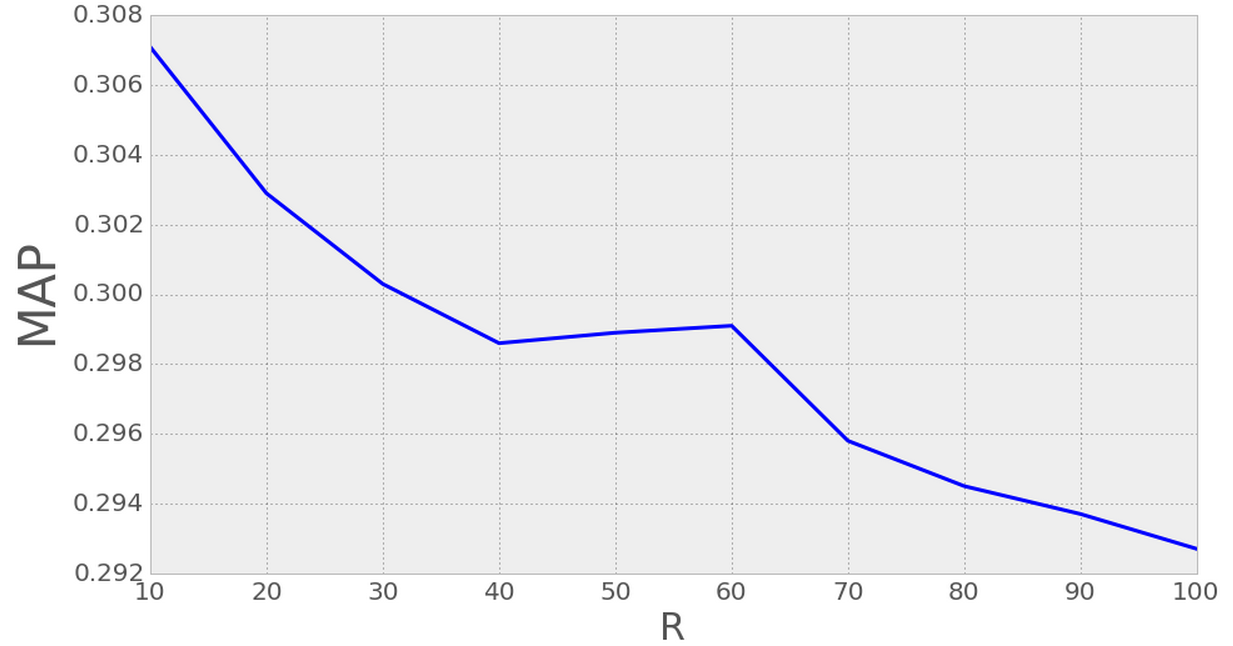
\includegraphics[width=\textwidth]{figures/lab4_R.png}
		\caption[Network2]%
		{{\small Laboratorio 4 (\textsc{rf pseudo}), al variare di $R$.}}    
		\label{fig:lab4_R}
	\end{subfigure}
	\hfill
	\begin{subfigure}[htpb]{0.475\textwidth}  
		\centering 
		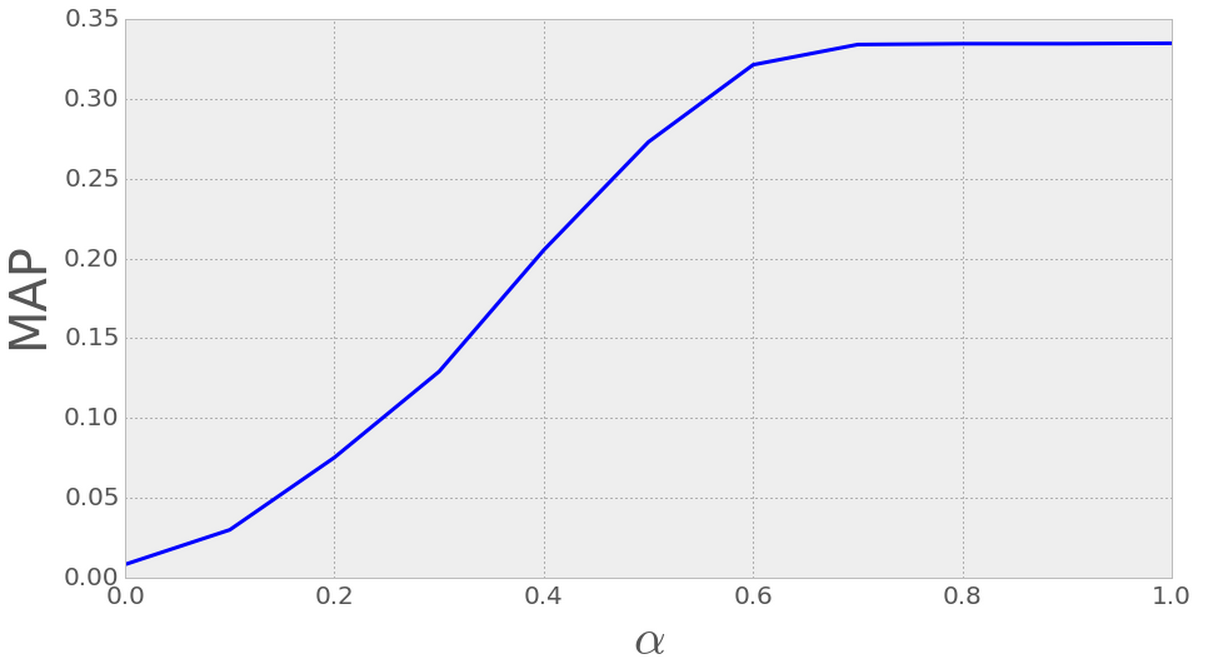
\includegraphics[width=\textwidth]{figures/lab5_alpha.png}
		\caption[]%
		{{\small Laboratorio 5 (\textsc{pagerank}), al variare di $\alpha$.}}    
		\label{fig:lab5_a}
	\end{subfigure}
	\vskip\baselineskip
	\begin{subfigure}[htpb]{0.475\textwidth}   
		\centering 
		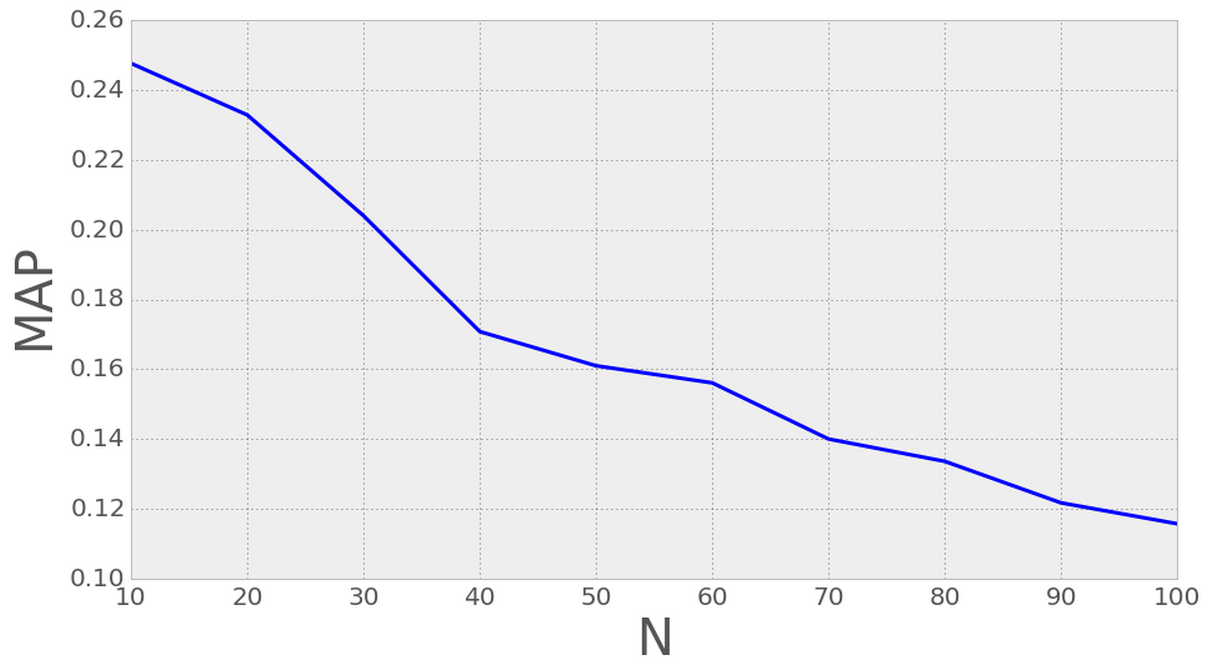
\includegraphics[width=\textwidth]{figures/lab6_N.png}
		\caption[]%
		{{\small Laboratorio 6 (\textsc{lsa}), al variare di $N$.}}    
		\label{fig:lab6_Nd}
	\end{subfigure}
	\quad
	\begin{subfigure}[htpb]{0.475\textwidth}   
		\centering 
		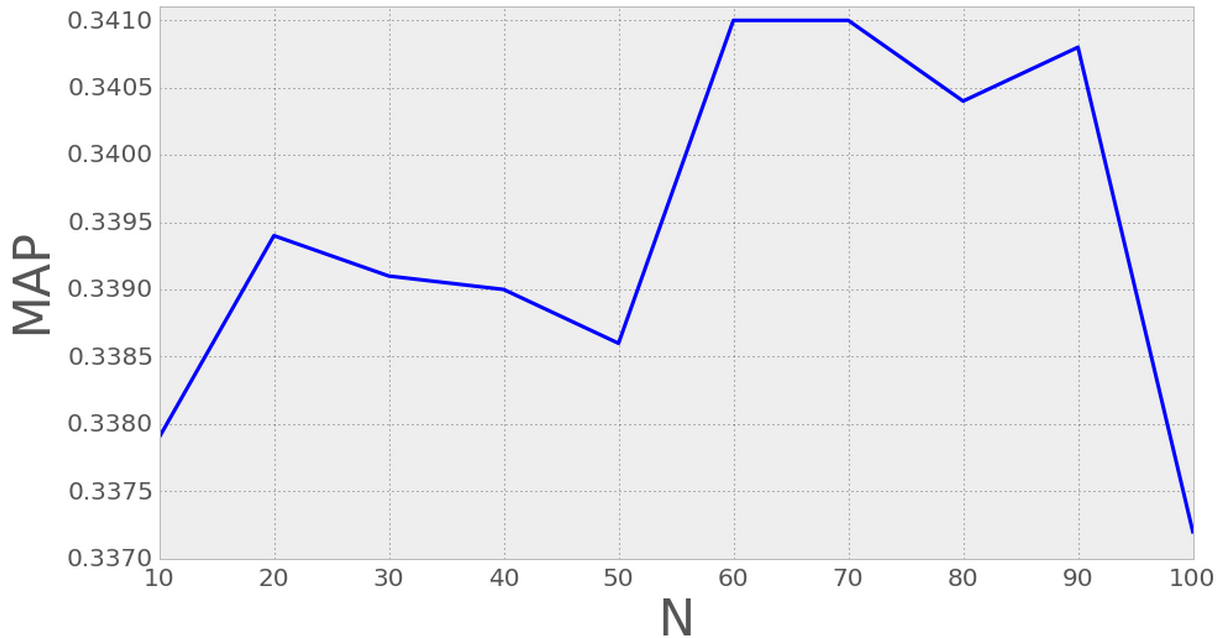
\includegraphics[width=\textwidth]{figures/lab7_N.png}
		\caption[]%
		{{\small Laboratorio 7 (\textsc{hits}), al variare di $N$.}}    
		\label{fig:lab7_Nd}
	\end{subfigure}
        \caption[ The average and standard deviation of claboratorioritical parameters ]
        {\small MAP al variare di alcuni parametri di configurazione della funzione di reperimento, per i diversi laboratori.} 
        \label{fig:map_all}
\end{figure*}
Come si pu\`o vedere da Figura \ref{fig:lab4_R} e Figura \ref{fig:lab6_Nd}, il \textsc{rf pseudo} e l'\textsc{lsa} peggiorano il valore della MAP al crescere del numero di documenti considerati rilevanti, e del numero di documenti da riordinare, rispettivamente. Ci\`o significa che dopo il primo passaggio di \textsc{bm25} l'ordine dei documenti \`e gi\`a preciso, e che l'effetto dello pseudo \textsc{rf} e di \textsc{lsa} \`e quello di alterare tale ordine, peggiorando l'efficacia del reperimento. In Figura \ref{fig:lab5_a} vediamo che $\alpha$ il parametro che regola l'influenza di \textsc{pagerank} sull'ordine dei documenti, ha un effetto molto negativo per valori piccoli, mentre migliora per valori pi\`u alti. Infine in Figura \ref{fig:lab7_Nd} vediamo che il reperimento che si avvale di \textsc{hits} ha un massimo per $N=60$, il che significa che se andiamo ad espandere un insieme radice di 60 elementi otteniamo in media la miglior MAP dopo il riordinamento.

Figura \ref{fig:map_hist} mostra le MAP dei vari metodi di reperimento a partire dalla configurazione \textsc{baseline} di \textsc{bm25} (laboratorio 3), scegliendo la miglior combinazione di parametri per ciascuno di essi. 
\begin{figure}[htpb]
	\begin{center}
		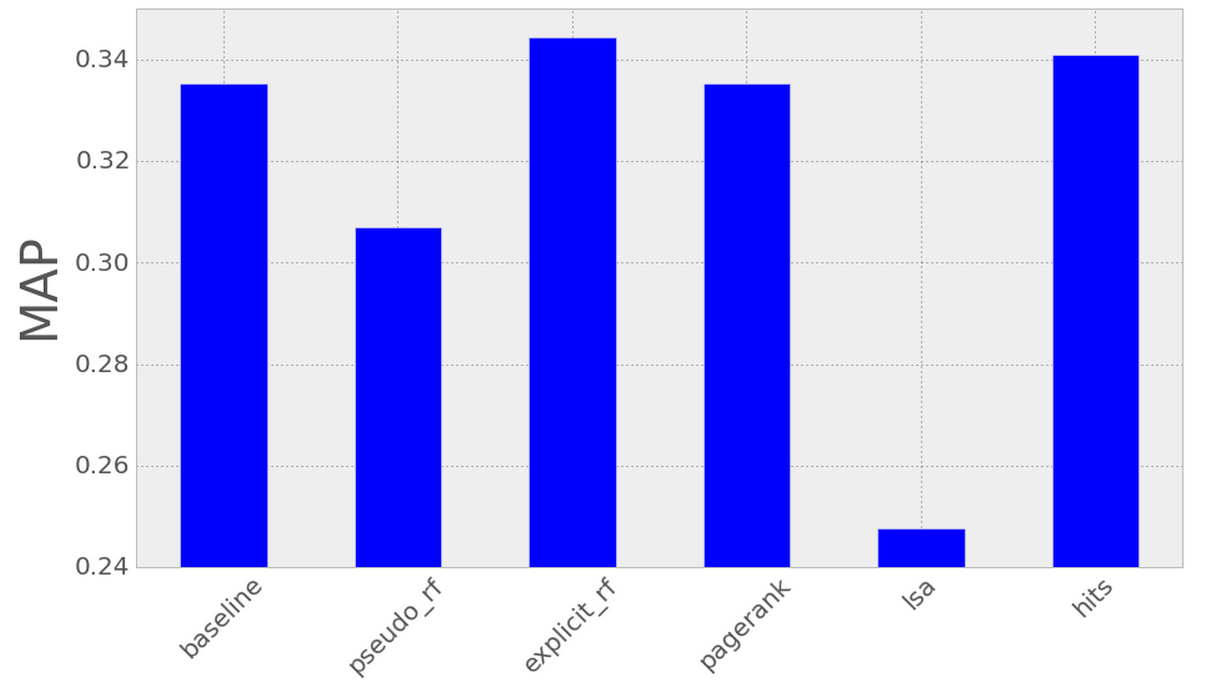
\includegraphics[width=0.75\textwidth]{figures/hist_map.png}
		\caption{MAP per i vari metodi di reperimento, a partire dai parametri di \textsc{bm25} della \textsc{baseline}.}
		\label{fig:map_hist}
	\end{center}
\end{figure}
Tabella \ref{tab:map} riporta i parametri usati per ogni funzione di reperimento e la relativa MAP ottenuta.
\begin{table}[htpb]
	\begin{center}
		\begin{tabular}{|c|c|c|}
			\hline
			metodo & parametri & MAP \\
			\hline
			\textsc{baseline} & - & $0.3354$ \\
			\textsc{rf esplicito} & - & $0.3445$ \\
			\textsc{rf pseudo} & $R=10$ & $0.3071$ \\
			\textsc{pagerank} & $\alpha=1.0$ & $0.3354$ \\
			\textsc{lsa} & $N=10, m=2$ & $0.2477$ \\
			\textsc{hits} & $\alpha=1.0, \beta=0.1, \gamma=0.1, N=60$ & $0.3410$ \\
			\hline
		\end{tabular}
	\end{center}
	\caption{Dettaglio dei parametri usati per le varie funzioni di reperimento e della relativa map. I parametri di \textsc{bm25} per ogni metodo sono quelli della \textsc{baseline} $k_1 = 0.0253, b = 0.0221$.}
	\label{tab:map}
\end{table}

Dai risultati riportati si pu\`o notare che gli unici metodi che hanno portato un miglioramento in termini di MAP rispetto alla \textsc{baseline}, sono l'uso del \textsc{rf esplicito}, e quello di \textsc{hits}. Il notevole peggioramento portato da \textsc{lsa} pu\`o essere spiegato dalla rappresentazione dei documenti nello spazio vettoriale, infatti essi contentendo molto pochi termini in media, sono vettori con molti elementi a zero. Ci\`o significa che nel nostro contesto, dopo la riduzione dimensionale, le similarit\`a tra i vettori non sono significative, e il riordinamento quindi sposta alcuni documenti rilevanti dalla cima della classifica verso il fondo. Per il \textsc{pagerank} invece possiamo vedere che sebbene esso non abbia portato un miglioramento partendo dai parametri della \textsc{baseline} (per $\alpha = 1$ il contributo di \textsc{pagerank} viene completamente ignorato nel reperimento), utilizzando $\alpha$ come parametro da ottimizzare, tale metodo pu\`o portare un leggero miglioramento della precisione, come riportato in Tabella \ref{tab:es}. In particolare, osservando che anche \textsc{hits} ha portato un aumento della MAP in questi termini, possiamo affermare che l'analisi del grafo delle citazioni porta informazione utile alla rilevanza.

\subsection{Efficienza}
\label{sec:efficienza}
Figura \ref{fig:efficiency} riporta i tempi di esecuzione delle varie funzioni di reperimento. I parametri utilizzati sono quelli riportati in Tabella \ref{tab:map}. Per ogni metodo si presume che l'indicizzazione sia gi\`a avvenuta, e inoltre tutte le misure calcolabili offline (a tempo di indicizzazione) siano gi\`a state computate (e.g. il dizionario, le lunghezze dei documenti, la document-term matrix, il valore di pagerank). Come si pu\`o vedere, in particolare grazie alla \textit{vectorization} usata per effettuare il calcolo di \textsc{bm25}, il tempo di esecuzione del reperimento \textsc{baseline} \`e molto breve, poco pi\`u di un secondo. 
\begin{figure}[htpb]
	\begin{center}
		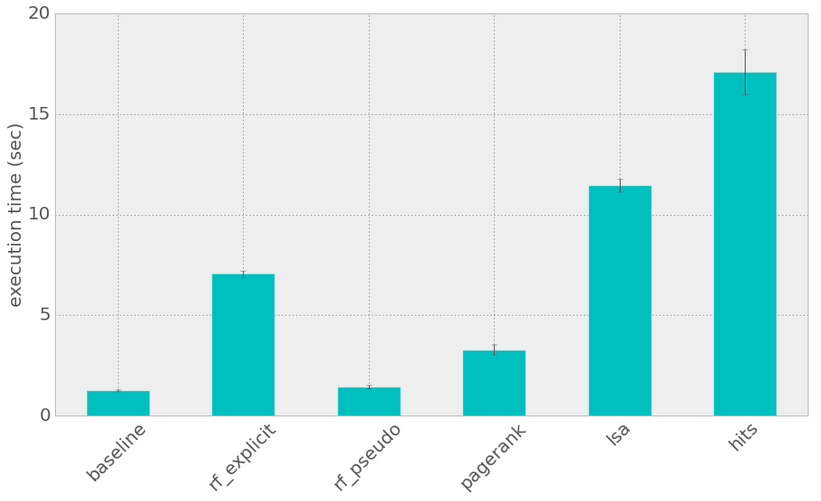
\includegraphics[width=0.75\textwidth]{figures/efficiency.png}
		\caption{Tempo di esecuzione (secondi) e relativa standard deviation per le varie funzioni di reperimento. Media su 20 run. Le run vengono eseguite su thread singolo.}
		\label{fig:efficiency}
	\end{center}
\end{figure}
Gli altri metodi di reperimento sono invece pi\`u impegnativi. In particolare, i metodi \textsc{lsa} e \textsc{hits} sono molto lenti, nel primo caso per la costosa decomposizione \textsc{svd} e il calcolo delle cosine similarity, nel secondo per l'espansione del grafo radice. Gli altri metodi hanno comunque dell'overhead dovuto ai tempi di lettura dei dati addizionali e al riordinamento della lista di documenti.

Tali risultati sono da considerarsi indicativi, in quanto non sono state usate regole vincolanti sul codice volte a garantire l'efficienza. Inoltre la dimensione della collezione  utilizzata ci ha permesso di effettuare maggior parte delle computazioni utilizzando matrici. Tale vantaggio non \`e applicabile al crescere del corpo di documenti.

%Questo paragrafo presenta e discute i risultati sperimentali. Si dovranno
%scegliere tre \textit{run} al massimo per ciascuno dei metodi illustrati nei
%paragrafi \ref{sec:metodi-di-reper}, \ref{sec:relevance-feedback},
%\ref{sec:pagerank}, \ref{sec:lsa} e \ref{sec:hits}.  
%
%Si dovranno confrontare le misure di efficacia (ad esempio, \textit{Mean Average
%  Precision}, MAP) mediante illustrazioni anche grafiche. Un'analisi della
%significativit\`a statistica delle differenze tra i valori di MAP sarebbe
%opportuna.
%
%Un confronto particolare dovr\`a essere fatto tra la \textit{baseline} del
%paragrafo \ref{sec:metodi-di-reper} e i metodi dei paragrafi successivi.
%
%La parte preziosa di questo paragrafo \`e la discussione dei risultati. Si
%dovr\`a dare un'interpretazione ragionata, chiara ed esaustiva delle ipotesi per
%cui sono state osservate o meno le differenze tra i valori di MAP. 



\section{Conclusioni}
\label{sec:conclusioni}
Nell'arco del corso di Sistemi Informativi sono state affrontate diverse tecniche per il reperimento. Durante le implementazioni abbiamo notato che non sempre metodi pi\`u avanzati portavano un miglioramento rispetto alla \textsc{baseline} e anche quando questo succedeva, la configurazione dei parametri era molto suscettibile e delicata. Inoltre la MAP ottenuta \`e relativamente bassa rispetto alle nostre aspettative iniziali. Siamo quindi arrivati a domandarci i motivi di questo comportamento. Analizzando il testo delle query abbiamo avuto modo di verificare come alcune di esse hanno bisogni informativi che riguardano informazioni che non sono presenti nel corpo di documenti indicizzati. Molte di esse chiedono infatti informazioni quali l'autore o l'anno di pubblicazione, altre invece esprimono regole di esclusione (eg. query 6: ``[...] We are not interested in the dynamics of arm motion.'') che non vengono considerate come tali dal modello che abbiamo utilizzato. Infine un altro aspetto che ha influenzato i risultati \`e il fatto che per molti documenti mancano gli abstract, e viene utilizzato solo il titolo. \`E difficile esprimere il vero contenuto informativo di un articolo utilizzando solamente le 2-10 parole del titolo. Riteniamo che questi fattori portino ad uno scarso miglioramento dell'efficacia del reperimento utilizzando tecniche avanzate, che potrebbero invece contribuire in maniera significativa su collezioni pi\`u grandi e complete. 

Abbiamo notato che alcune query sono formulate in modo molto colloquiale; queste situazioni portano ad avere degli stem che non descrivono in modo appropriato il bisogno informativo dell'utente. Un chiaro esempio \`e la query 64: ``List all articles on EL1 and ECL (EL1 may be given as EL/1; I don't remember how they did it.'' riassunta con gli stem \textit{[articl, ecl, el, list, rememb]}. In questo caso lo stem \textit{rememb} non ha senso perch\`e appartiene ad un commento personale dell'utente, per\`o \`e uno dei 5 stem che descrivono la query.

Sarebbe interessante sperimentare ulteriori tecniche di elaborazione delle query; ad esempio l'implementazione di QE (Query Expansion) potrebbe ridurre il fenomeno del \textit{topic drift} (interrogazioni fuori tema) presente in alcune query.

Abbiamo avuto modo di verificare il notevole miglioramento della MAP utilizzando \textsc{rf esplicito}, che non risente pesantemente di queste considerazioni, in quanto modifica l'ordinamento basandosi solamente su informazioni di rilevanza e occorrenze dei termini, e non utilizza aspetti pi\`u elaborati (e.g.: il grafo delle citazioni).

Un altro aspetto \`e stato gestire l'efficienza del reperimento. Sarebbe interessante verificare in che modo le tecniche realizzate si comportano con l'utilizzo di collezioni pi\`u grandi, e quali delle scelte effettuate per le implementazioni sulla collezione CACM si rivelano essere dei colli di bottiglia al crescere del corpo di documenti.

\bibliographystyle{abbrv}
\bibliography{references}

%In questo paragrafo si possono aggiungere delle osservazioni di carattere
%generale sugli esperimenti; ad esempio, si pu\`o concludere se un proprio metodo
%di reperimento o una variazione dei metodi pi\`u avanzati hanno portato a
%qualche miglioramento rispetto alla \textit{baseline}.

\end{document}
